	\section{薛定谔方程}
		在量子力学中的作用和逻辑等价于经典力学中的牛顿定律:给定适当的初始条件,薛定谔方程决定以后所有时刻的波函数$\Psi (x,t)$
	\section{波函数的统计诠释}
		波恩关于波函数的统计诠释给出,$|\Psi (x,t)|^2$给出时刻t在x处发现粒子的几率,更准确的说
		\begin{equation}
			\int_{a}^{b}|\Psi(x, t)|^{2} d x
		\end{equation}
		在t时刻发现粒子处于a和b之间的几率

		这里有三种学派回答测量和粒子位置之间的关系
		\begin{enumerate}
		\item 现实主义学派:意味着量子力学本身就是不完备的,即量子力学本身的缺陷导致无法告知粒子准确的位置————需要隐变量提供附加信息才能完成对粒子的完整描述。
		\item 哥本哈根(Copenhagen)学派,即粒子本就“无处不在”,是观测行为“强迫”粒子出现在特定的位置————但是这样,测量的作用将变得非常的独特,我们将在后续处理这件事情。\footnote{Unfinished.}
		\item 不可知论学派:即拒绝回答。即无法定义怎样的行为才能够称为测量,那么测量前和测量后的状态也无法被准确的定义,这时候讨论其本质已经是不可能的。
		\end{enumerate}
		
		最新的实验为哥本哈根学派的观点做出了较强的支撑:\textbf{一个粒子在测量前没有一个确定的位置,就像水面的波纹,是测量的过程给出了一个具体数量,在这个意义上,给出了受波函数统计权重限定的特定的结果。}连续两次测量(即时间间隔较短)的结果是相同的,事实是第一次测量完全改变了波函数,如图\ref{fig.WavefunctionCollapse}所示, 所以它现在是尖锐的在C点耸起我们称之为由于测量产生的波函数的坍塌。
		\begin{figure}[H]
			\centering
			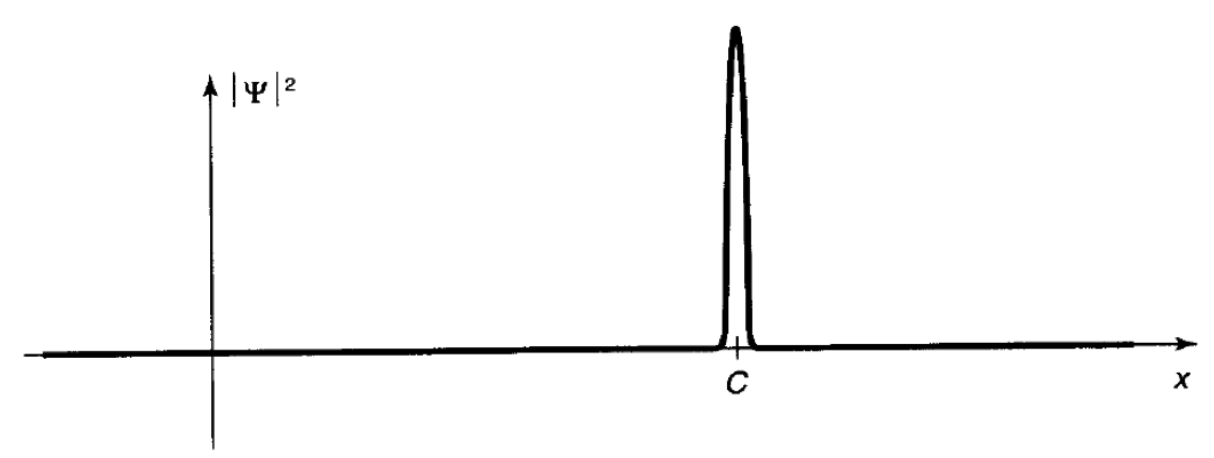
\includegraphics[width=0.5\linewidth]{sections/fig/WavefunctionCollapse.png}
			\caption{波函数坍缩示意图} 
			\label{fig.WavefunctionCollapse}
		\end{figure}
	\section{概率}
		已知j的概率分布,定义j的函数的平均值
		\begin{equation}
		\langle f(j)\rangle=\sum_{0}^{\infty} f(j) P(j)
		\end{equation}
		给出方差的定义和重要的一个定理
		%方差equ
			\begin{equation}
			\sigma^{2} \equiv\left\langle(\Delta j)^{2}\right\rangle
			\end{equation}
			\begin{equation}
			\begin{aligned}
			\sigma^{2} &=\left\langle(\Delta j)^{2}\right\rangle=\sum(\Delta j)^{2} P(j)=\sum(j-\langle j\rangle)^{2} P(j) \\
			&=\sum\left(j^{2}-2 j\langle j\rangle+\langle j\rangle^{2}\right) P(j) \\
			&=\sum j^{2} P(j)-2\langle j\rangle \sum j P(j)+\langle j\rangle^{2} \sum P(j) \\
			&=\left\langle j^{2}\right\rangle-2\langle j\rangle\langle j\rangle+\langle j\rangle^{2}=\left\langle j^{2}\right\rangle-\langle j\rangle^{2} .
			\end{aligned}
			\end{equation}
		上式取平方根,有$\sigma=\sqrt{\left\langle j^{2}\right\rangle-\langle j\rangle^{2}}$
	\section{归一化}
		波函数的统计诠释要求下式必须成立
		\begin{equation}
			\int_{-\infty}^{\infty}|\Psi(x, t)|^{2} d x=1
		\end{equation}
		薛定谔方程本身有着不同的特性,会自动保持波函数的归一化,下面给出证明:

		我们首先计算
		\begin{equation}
		\label{eq.1_1_0}
			\frac{d}{d t} \int_{-\infty}^{\infty}|\Psi(x, t)|^{2} d x=\int_{-\infty}^{\infty} \frac{\partial}{\partial t}|\Psi(x, t)|^{2} d x
		\end{equation}
		根据偏导数给出方程右边形式:
		\begin{equation}
		\label{eq.1_1_1}
			\frac{\partial}{\partial t}|\Psi|^{2}=\frac{\partial}{\partial t} \Psi^{*} \Psi=\Psi^{*} \frac{\partial \Psi}{\partial t}+\frac{\partial \Psi^{*}}{\partial t} \Psi
		\end{equation}
		将薛定谔方程写做
		\begin{equation}
			\frac{\partial \Psi}{\partial t}=\frac{i \hbar}{2 m} \frac{\partial^{2} \Psi}{\partial x^{2}}-\frac{i}{\hbar} V \Psi
		\end{equation}
		同时给出方程复共轭的形式
		\begin{equation}
			\frac{\partial \Psi^{*}}{\partial t}=-\frac{i \hbar}{2 m} \frac{\partial^{2} \Psi^{*}}{\partial x^{2}}+\frac{i}{\hbar} V \Psi^{*}
		\end{equation}
		代入式\ref{eq.1_1_1}可得
		\begin{equation}
		\label{eq.1_1_psi^2dt}
			\frac{\partial}{\partial t}|\Psi|^{2}=\frac{i \hbar}{2 m}\left(\Psi^{*} \frac{\partial^{2} \Psi}{\partial x^{2}}-\frac{\partial^{2} \Psi^{*}}{\partial x^{2}} \Psi\right)=\frac{\partial}{\partial x}\left[\frac{i \hbar}{2 m}\left(\Psi^{*} \frac{\partial \Psi}{\partial x}-\frac{\partial \Psi^{*}}{\partial x} \Psi\right)\right]
		\end{equation}
		则式\ref{eq.1_1_0}可直接写做
		\begin{equation}
			\frac{d}{d t} \int_{-\infty}^{\infty}|\Psi(x, t)|^{2} d x=\left.\frac{i \hbar}{2 m}\left(\Psi^{*} \frac{\partial \Psi}{\partial x}-\frac{\partial \Psi^{*}}{\partial x} \Psi\right)\right|_{-\infty} ^{\infty}
		\end{equation}
		即要求$x$趋于正负无限大的时候$\Psi (x,t)$必须趋于零————否则波函数式不可归一化的,所以得到
		\begin{equation}
			\frac{d}{d t} \int_{-\infty}^{\infty}|\Psi(x, t)|^{2} d x=0
		\end{equation}
	\section{动量}
		对于处于$\Psi$态的粒子(即处于“未观测态”的粒子),其x的期待值是
		\begin{equation}
		\label{eq.<x>}
		\langle x \rangle = \int_{-\infty}^{+\infty}x|\Psi (x,t)|^2 d x
		\end{equation}
		值得注意的是,这里不意味着对同一体系进行重复测量得到的平均值,而是对含有相同体系的一个系综中的不同体系的重复测量的平均值————如果对同一体系进行重复测量,第一次测量将导致分布的波函数坍缩。

		在函数随时间演化的过程中,我们更对$\langle x \rangle$发生的变化感兴趣,联立式\ref{eq.1_1_psi^2dt}和式\ref{eq.<x>},得到
		\begin{equation}
		\frac{d \langle x \rangle}{dt}=\int x \frac{\partial}{\partial t}|\Psi|^2 dx=\frac{i \hbar}{2m}\int x\frac{\partial}{\partial x}(\Psi^* \frac{\partial \Psi}{\partial x}-\frac{\partial \Psi^*}{\partial x}\Psi)dx
		\end{equation}
		利用分部积分公式得到\footnote{Unfinished}
		\begin{equation}
		\frac{d\langle x\rangle}{d t}=-\frac{i \hbar}{2 m} \int\left(\Psi^{*} \frac{\partial \Psi}{\partial x}-\frac{\partial \Psi^{*}}{\partial x} \Psi\right) d x
		\end{equation}
		对于上式,利用$\frac{\partial x}{\partial x}=1$,并丢掉了边界项,因为在无穷远处趋于零,再次分布积分得到
		\begin{equation}
		\langle v \rangle = \frac{d\langle x\rangle}{d t}=-\frac{i \hbar}{m} \int \Psi^{*} \frac{\partial \Psi}{\partial x} d x
		\end{equation}

		这里得到的是x期待值的“速度”。在量子力学中,本来就没有一个确切的速度定义————如果一个粒子没有一个确定的位置,就没有一个明确定义的速度,我们只能得到一个特定值的几率。

		在习惯中,我们使用动量表示:
		\begin{equation}
		\langle p \rangle = m \frac{d \langle x \rangle}{dt}=-i \hbar \int(\Psi^* \frac{\partial \Psi}{\partial x})dx
		\end{equation}
		我们把$\langle x \rangle$和$\langle p \rangle$的表示式写成更有启发意义的形式:
		\begin{equation}
		\begin{aligned}
		&\langle x\rangle=\int \Psi^{*}(x) \Psi d x \\
		&\langle p\rangle=\int \Psi^{*}\left(\frac{\hbar}{i} \frac{\partial}{\partial x}\right) \Psi d x
		\end{aligned}
		\end{equation}
		比较两个式子,我们可以发现计算任意量的期待值都可以将相应的算符放在$\Psi^*$和$\Psi$之间,然后求相应的积分,具体例子如下式\ref{eq.1_2_0}

		知道了位置和动量的量子力学表达,其他所有的经典力学量都可以表示为坐标和动量的函数。要计算这样的一个量的期待值,可以通过式
		\begin{equation}
		\label{eq.1_2_0}
		\langle Q(x, p)\rangle=\int \Psi^{*} Q\left(x, \frac{\hbar}{i} \frac{\partial}{\partial x}\right) \Psi d x
		\end{equation}

		请读者尝试求出动能的期待值\footnote{答案是
		\begin{equation}
		\langle T\rangle=-\frac{\hbar^{2}}{2 m} \int \Psi^{*} \frac{\partial^{2} \Psi}{\partial x^{2}} d x
		\end{equation}}

	\section{不确定原理}
		在直观感受上格里菲斯版的量子力学中给出的\textbf{绳的类比}相当的直观。\begin{figure}[H]
				\centering
				\subfigure[具有很好的波长定义,但是位置无法确定]{
				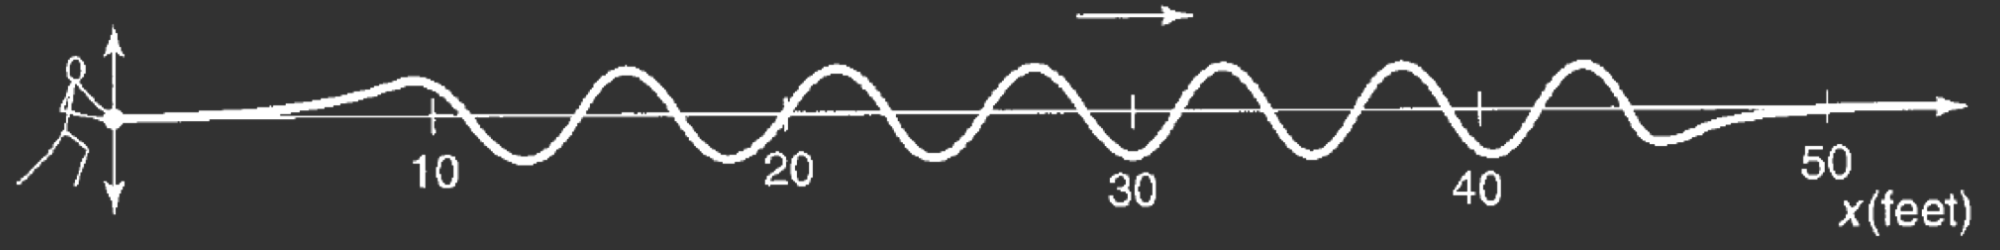
\includegraphics[width=0.7\linewidth]{sections/fig/UncertaintyI.png}
				}
				\quad
				\subfigure[具有很好的位置定义,但是波长无法定义]{
				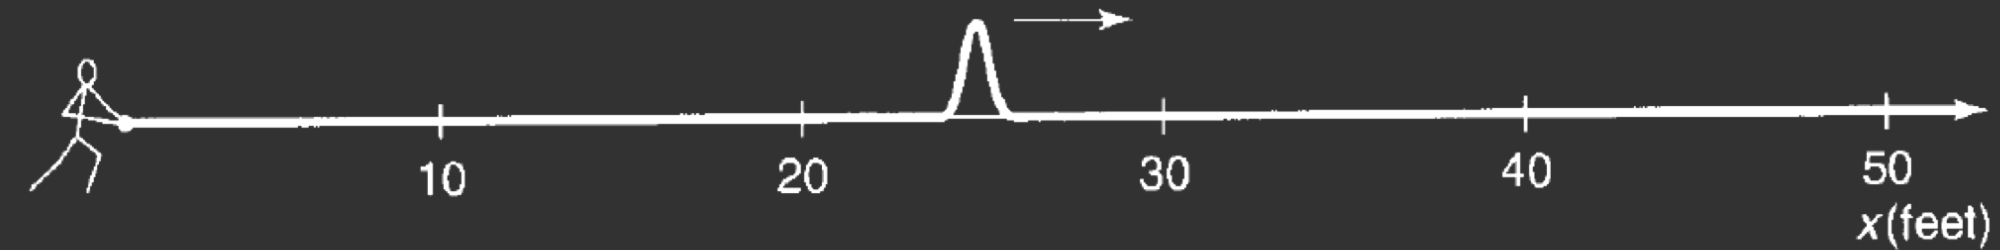
\includegraphics[width=0.7\linewidth]{sections/fig/UncertaintyII.png}
				}
				\caption{不确定性原理}
				\end{figure}

		粒子的动量同$\Psi$波长的联系由德布罗意公式给出。在这里我们不加证明的给出Heisenberg不确定原理,我们将在后面证明这个关系\footnote{Unfinished},在定量上有(其中中$\sigma_x$和$\sigma_p$分别是x和p的标准差)
			\begin{equation}
			\sigma_{x} \sigma_{p} \geq \frac{\hbar}{2}
			\end{equation}